\section{Fundamentals and Related Work} \label{fundamentals}

\subsection{From Probabilistic Language Models to modeling Evolution Theory} \label{fundamentalsA}

A probabilistic language model tries to approximate the probability distribution 

\begin{equation}
	P(w_1, ..., w_n) = \Pi_{t=1}^{n} P(w_t | w_1, ..., w_{t-1})
\end{equation}

with $w_t$ being a word at position (timestamp) $t$ in a sentence of length $n$. To build language models \acp{RNN} were used to model such probability distributions. 

\begin{figure}[ht]
	\centering
	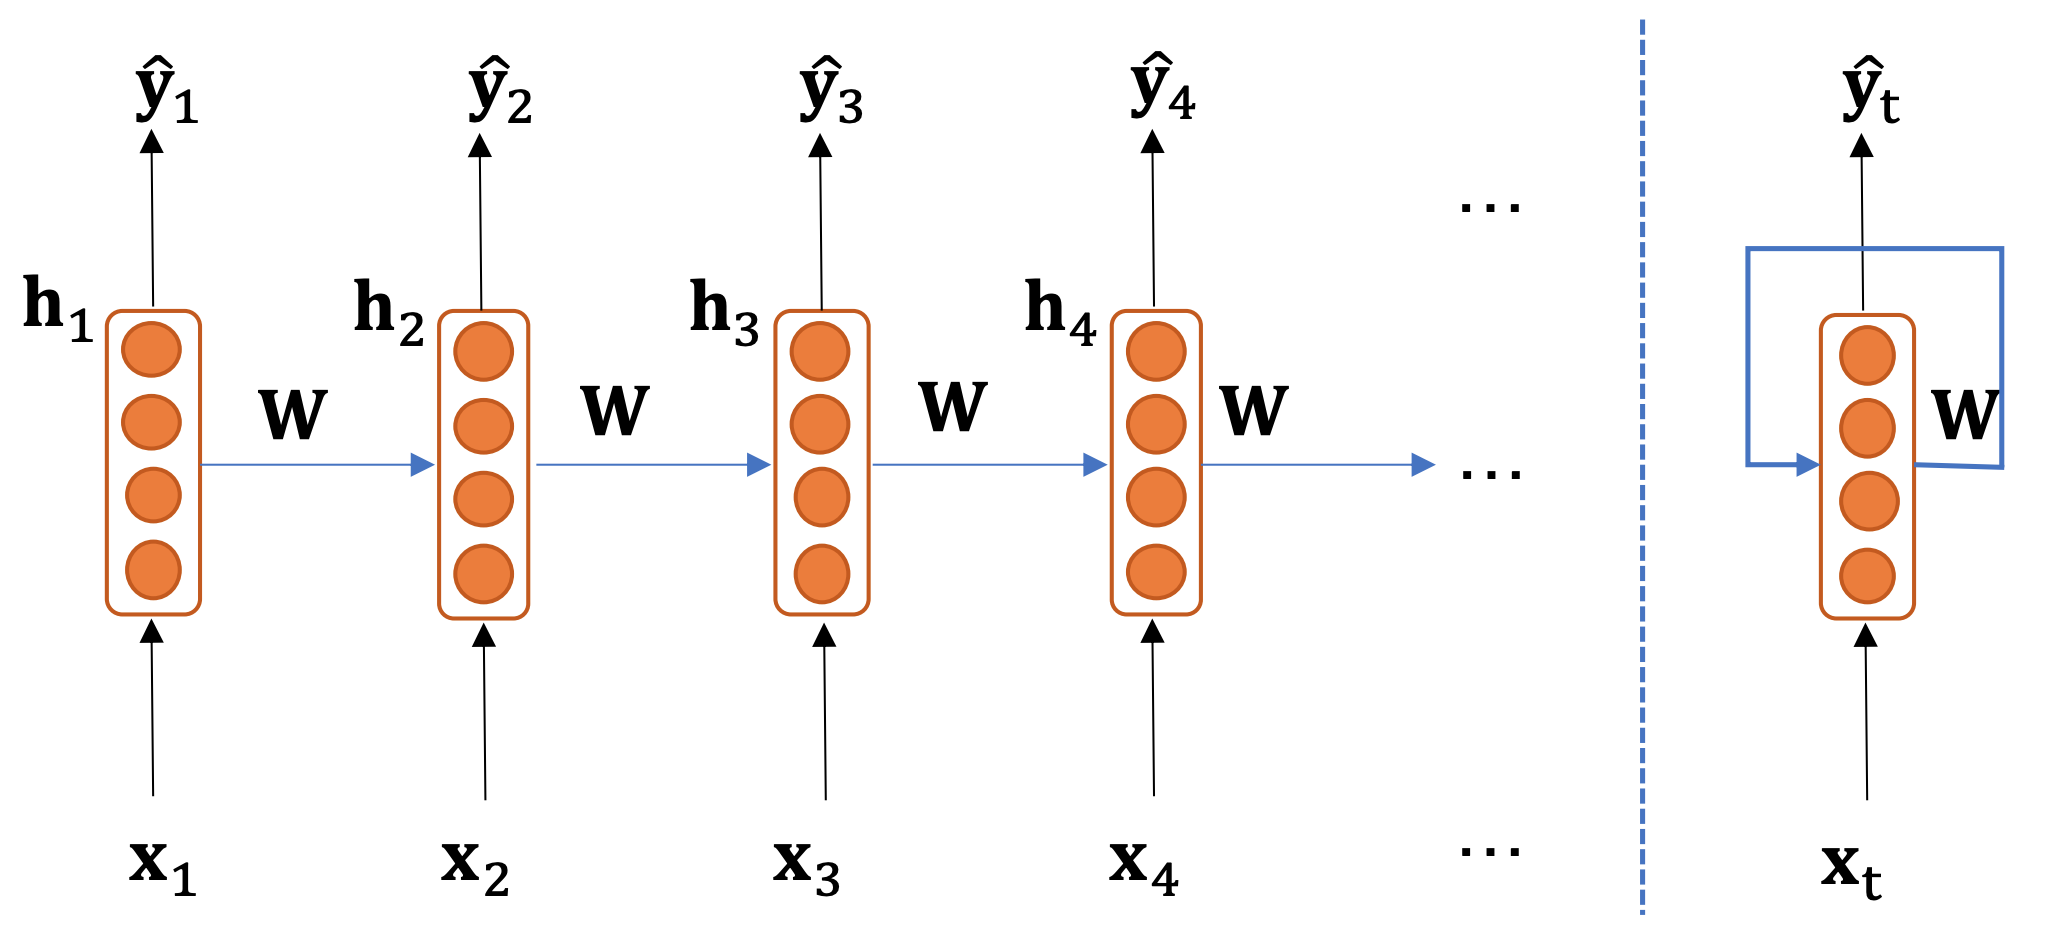
\includegraphics[width=0.8\linewidth]{figures/rnn_architecture.png}
	\caption{Architecture of a conventional \ac{RNN} model \cite{Gertz2020}}
	\label{rnn_architecture}
\end{figure}

At each time step $t$ it outputs a probability distribution $P(w_t | w_1, ..., w_{t-1})$ given the words read so far in the current instance (see \autoref{rnn_architecture}). Words are read as a vectorized numerical representation, often so-called word embeddings $x_t$. One then calculates the hidden state $h_t$ by

\begin{equation}
	h_t = f(W^{(h)} h_{t-1} + W^{(x)} x_t + b_1)
\end{equation}

and the corresponding output porbability distribution by 

\begin{equation}
	\hat{y}_t = softmax(U^{(h)} h_t + b_2).
\end{equation}

The applied weight matrix is always the same for each time step $t$ giving the \ac{RNN} its name. One can therefore simplify the unrolled \ac{RNN} architecture on the left side of \autoref{rnn_architecture} to the one on the right, where the hidden state is continuously passed as an input to the next time step. To achieve a better convergence behavior during training, one can also provide the expected hidden state of time step $t-1$ instead of using the predicted hidden state, which is called teacher forcing. \acp{RNN} are able to process input of arbitrary length and are by their recurrent character capable to use information from previous time steps. Unfortunately, they are vulerable to vanishing and exploding gradient problems. \ac{LSTM} is a special \ac{RNN} architecture that solves such vulnerabilities by owning a separate long-term cell state besides a short-term hidden state and is introduces in \autoref{fundamentalsE}. It is able to preserve information over many time steps. \cite{Gertz2020}

\begin{figure}[ht]
	\centering
	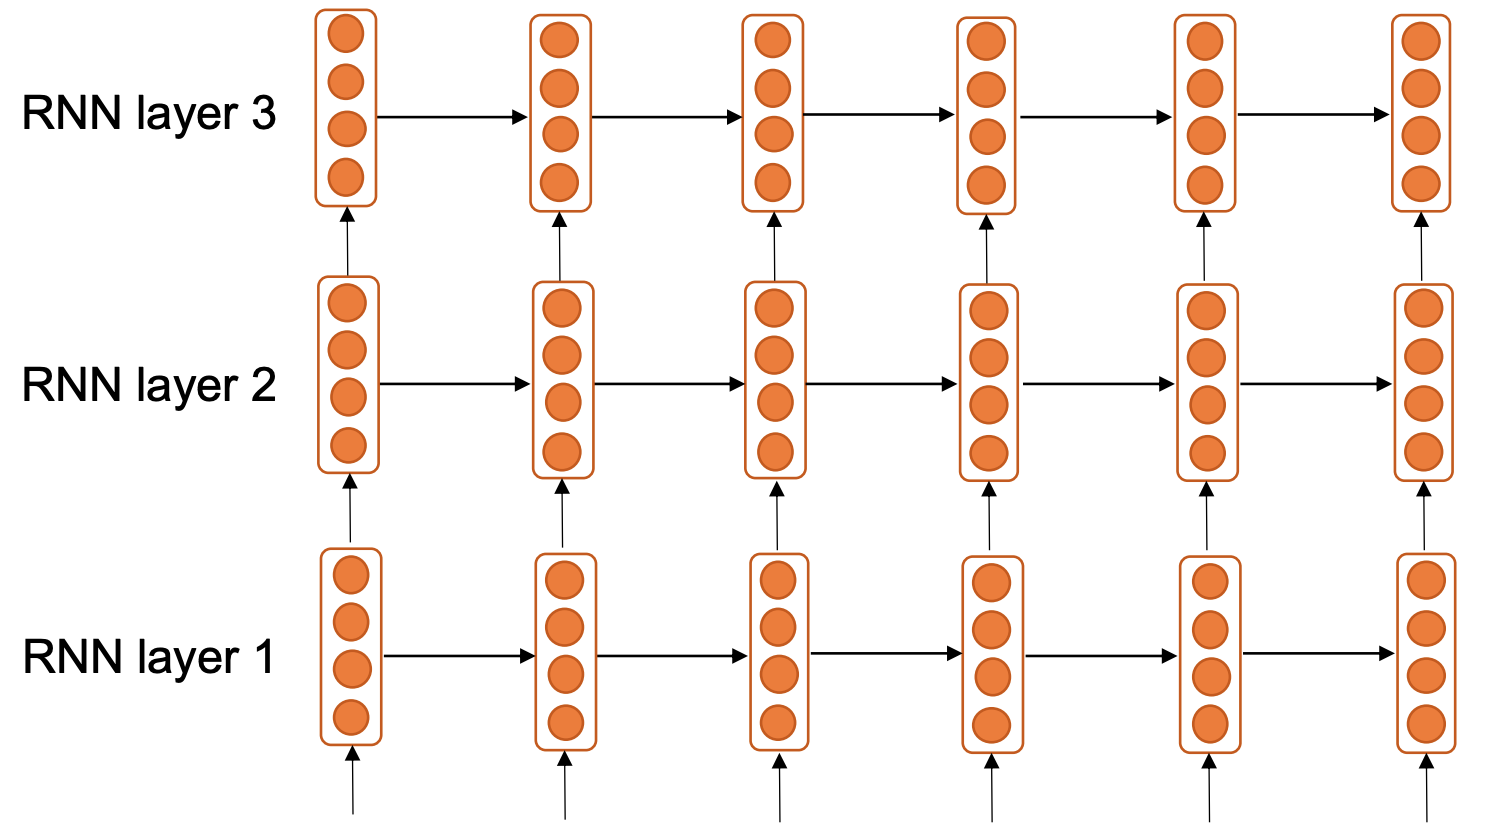
\includegraphics[width=0.8\linewidth]{figures/multi_layer_rnn.png}
	\caption{Architecture of a multi-layer  \ac{RNN} \cite{Gertz2020}}
	\label{multi_layer_rnn}
\end{figure}

One can also use two \acp{RNN}, one traversing a sentence from left to right and another one vice versa, with two different weight matrices to model the probability distribution bidirectionally. One therefore simply concatenates the hidden states of each \ac{RNN} before applying the the weight matrix $U$ and the $softmax()$ function. Also multi-layer \acs{RNN} can be utilized to generate higher-order features (hidden states) for the prediction task (see \autoref{multi_layer_rnn}). \cite{Gertz2020}

The \acp{RNN} or even better \acp{LSTM} architectures used for probabilistic language modeling can be reused in a more complex domain called sequence to sequence modeling for neural machine translation from one language to another. Here one first tries to learn a fixed-dimensional input representation from an input sequence using an encoder architecture based on an \ac{LSTM}. The so-called context vector is then decoded by a second \ac{LSTM} into a new sequence of words preserving the grammar but owning a different meaning. \cite{Sutskever2014}

Sequence to sequence models are introduced together with the \ac{LSTM} architecture in \autoref{fundamentalsE}. Here the connection to evolution theory can be drawn. \ac{RNA} sequences made of a concatenation of nucleotides \footnote{We restrict the representation of nucleotides solely to their nucleobases parts consisting of the distinct nucleobases guanine, adenine, cytosine and thymine. We therefore do not include the phosphate group and the five-carbon sugar components.} can be represented textually using the FASTA format. A sequence to sequence model can then transferably be applied in the domain of \ac{RNA} sequences to model how \ac{RNA}-based viruses change their structure to avoid the detection by the human immune system but still to preserve their infectivity and evolutionary fitness \cite{Hie2021}. 

\subsection{GISAID EpiFlu Data Platform} \label{fundamentalsB}

\subsection{Domain-Specific Methodologies to create Evolutionary  Datasets for Mutation Prediction} \label{fundamentalsC}

\subsection{Previous Work on Mutation Prediction} \label{fundamentalsD}

Even before the rise of Covid-19 there had been studies trying to predict mutations of RNA viruses. In the collection of \cite{Wu2007, Yan2007, Wu2008} the authors predict the mutation positions in hemagglutinins from influenza A virus using logistic regression and plain neural networks and then use the resulting amino acid mutating probabilities to derive possible mutated amnio acids. The same approach is further used for H5N1 neuraminidase proteins. 

\cite{Salama2016} proved that nucleotides in an RNA sequence can change based on their local neighborhood. Neural networks are used to predict new strains of the Newcastle virus and subsequently a rough set theory based algorithm is introduced to extract the according point mutation patterns. 

\cite{Mohamed2021} uses a more modern sequence to sequence  \ac{LSTM} approach to learn nucleotide mutations between time-series species of H1N1 Influenza virus and the Newcastle virus as mutations can also be influenced by long-distance relations of amino acids. Therefore one hot-encoded RNA sequences of a parent generation preprocessed to words is given as an input and the output is the predicted offspring generation evaluated by accuracy to the compared true offspring generation. The achieved accuracy in this paper is questionably high with 98.9\% on the H1N1 Influenza virus and 96.9\% on the Newcastle virus, possibly because of overfitting to the few 4.609 samples for H1N1 Influenza virus and only 83 for the Newcastle virus. Our approach therefore tries to increase the number of samples available for training when building the dataset. 

Our approach will neither use any of the just mentioned architectures, but uses a Transformer based architecture coupled with a GAN-style training architecture. Nevertheless a short introduction into sequence to sequence models and the underlying long short-term memory components shall be given to better point out our architectural decisions . 

\subsection{Sequence2Sequence Models based on Long Short-Term Memory} \label{fundamentalsE}

% Figure Seq2Seq/LSTM

The original \ac{LSTM} unit was introduced in \cite{Hochreiter1997} and can be used for language modeling instead of using plain \acp{RNN} to prevent running into vanishing or exploding gradient problems \cite{Sundermeyer2012}. 



\cite{Sutskever2014} introduced sequence to sequence learning by using one \ac{LSTM} as an encoder to learn a large fixed-dimensional vector representation of the input and another \ac{LSTM} as a beam search decoder to map the so-called context vector, the last hidden state after processing the entire input, to a corresponding output sequence whose length does not need to match with the length of the input sequence. The output sequence is therefore given by the equation

\begin{equation}
	p(y_1, ..., y_{T'} | x_1, ..., x_{T}) = \Pi_{t=1}^{T'} p(y_t | v, y_1, ..., y_{t-1})
\end{equation}

with $v$ being the context vector. Using an \ac{LSTM} is prefered over a normal \ac{RNN} as it is used to capture the long range temporal dependencies of the input data, each \ac{LSTM} uses four layers with 1000 cells each. One finding was also that reversing the input sequence introduces many short term dependencies making optimization easier. The sequence to sequence model approach was evaluated for neural machine translation and reached a 34.81 BLEU score with an output vocabulary of 80k words (160k words input vocabulary, 1000 dimensional word embeddings, 8000 real numbers to represent a sentence). 

% From Hindawi: Each LSTM cell takes information as input from the previous cell, in the form of a hidden state vector and cell state vector (represented in arrows) and combines it with the one-hot encoded vector. The output of the encoder is the concatenation of the hidden and cell-state vectors. In the decoder, each cell receives as input [i] in the one-hot encoded version and the previous word of the next generation generated by the model, as well as the hidden state and cell-state vectors from the previous cell. It not only passes those two vectors after updating them to the next cell but also feeds the hidden state vector to the dense layer (output layer), which outputs a probability distribution over the next generation word at that position. A SoftMax function is applied to obtain probability distribution. To reduce overfitting, early stopping is used to end training when the validation loss did not decrease.

\subsection{Applying Generative Adversarial Networks} \label{fundamentalsF}

\begin{itemize}
	\item Covid-Paper: \url{https://arxiv.org/pdf/2008.11790.pdf}
\end{itemize}


\subsection{Transformer and Attention Mechanism} \label{fundamentalsG}

\begin{itemize}
	\item Improvement: \url{https://arxiv.org/abs/1706.03762}
\end{itemize}


\subsection{Other Techniques} \label{fundamentalsH}

\begin{itemize}
	\item NNs/SVMs: \url{https://bsb-eurasipjournals.springeropen.com/articles/10.1186/s13637-016-0042-0}
	\item BiLSTM: \url{https://science.sciencemag.org/content/371/6526/284}
\end{itemize}


\newpage
